% Supporting information for upgrade report
\documentclass[11pt]{article}
\usepackage{graphicx}
\usepackage[margin = 2.5cm]{geometry}
\usepackage[T1]{fontenc}
\usepackage{setspace}
\usepackage{xcolor}

% captions
\usepackage[labelfont=bf]{caption} 
\captionsetup{skip=7pt} 
\captionsetup[figure]{font=footnotesize}
\captionsetup[table]{font=footnotesize}
\captionsetup{font=footnotesize,font={stretch=1}}

% subfigures and subcaptions
\usepackage{subcaption}  

% tables
\usepackage{multirow}
%\usepackage{longtable} 
\usepackage{array}
%\usepackage{verbatim} 

%Line numbering
\usepackage{lineno}

% clinkable links 
\usepackage[hidelinks]{hyperref}
\hypersetup{
    colorlinks=false, %set true if you want colored links
    linktoc=all     %set to all if you want both sections and subsections linked
    %linkcolor=blue,  %choose some color if you want links to stand out
}

% useful to comment out large sections:
\usepackage{verbatim} 

% line spacing
%\renewcommand{\baselinestretch}{2}



\begin{document}

\title{\textbf{Supporting information for\\
\vspace{1cm}
The influence of vertebrate species traits on their responses to land-use and climate change
\vspace{2cm}}}

\author{Adrienne Etard}

\maketitle

% CONTENTS
\clearpage
\tableofcontents

%\cleardoublepage
%\addcontentsline{toc}{section}{List of Tables}

\clearpage
\listoftables
%\addcontentsline{toc}{section}{List of Figures}

\clearpage
\listoffigures

% \clearpage
% List of abbreviations

\clearpage

\section{Trait data compilation}

\subsection{Habitat affinities and broad specialisation}
\paragraph{Habitat preferences.}
% Pooling in broader habitat categories
IUCN habitat data records habitat types in which species occur. Habitats are classified into 96 categories, which I pooled into 13 broader habitat variables: 
Forest, Savanna, Grassland, Shrubland, Wetland, Rocky areas, Caves and subterranean, Desert, Marine, Marine intertidal or coastal/supratidal, Artificial, Introduced vegetation and Other/Unknown. Species habitat preferences were described using these variables as binary (taking 1 if a species was known to occur in the habitat and 0 otherwise).
\paragraph{Habitat breadth.}
Habitat breadth was calculated as the number of habitats recorded to be used by a species in the IUCN database. Given that information regarding habitat suitability and habitat importance was also available in the IUCN data files, I used a weighted sum to calculate habitat breadth. Suitability was declined in three categories in the IUCN files: `suitable', `marginal' or  `unknown'. Habitats were recorded to be either of major importance, not of major importance or of unknown importance. I used the weights provided in Table \ref{weights} to produce weighted sums of the number of habitats used by each species. A comparison of the distribution of habitat breadths calculated with and without weights shows that weighting did not have a strong impact on the results (Figure \ref{distHB}).

% table of weigths used for habitat breadth calculations
\begin{table}[h!]
\renewcommand{\baselinestretch}{1}
\renewcommand{\arraystretch}{1.5}
\begin{center}\fontsize{9}{11}\selectfont
\caption[Weights used in the calculation of habitat breadth]{\textbf{Weights used in the calculation of habitat breadth.} Habitat breadth was calculated as the weighted sum of the number of habitats used by a species. Weights were assigned to each habitat given its importance and its suitability.} 
\label{weights}
\begin{tabular}{|l|c|c|c|}
\hline
\multicolumn{1}{|c|}{\multirow{2}{*}{\textbf{Suitability}}} & \multicolumn{3}{c|}{\textbf{Major importance}} \\ \cline{2-4} 
\multicolumn{1}{|c|}{}                             & \textbf{Yes}       & \textbf{No}        & \textbf{Unknown}       \\ \hline
\textbf{Suitable}                                           & 1         & 0.5       & 1             \\ \hline
\textbf{Marginal}                                           & 0.3       & 0.3       & 0.3           \\ \hline
\textbf{Unknown}                                            & 1         & 0.3       & 1             \\ \hline
\end{tabular}
\end{center}
\end{table}

% figure distribution of habitat breadths
\begin{figure}[h!]
\centering
\includegraphics[scale=0.8]{figures/Weighted_HB/distributions}
\caption[Distribution of habitat breadths across species for terrestrial vertebrates]{\textbf{Distribution of habitat breadths across species for terrestrial vertebrates.} The distribution is shown for calculations assigning weights to habitats according to their suitability and their importance (red surface area) or without weights (blue surface area). The distribution of habitat breadths slightly shifts to the left when a weighted sum is used (in \textbf{A}, \textbf{B} and \textbf{C}), as less importance is accorded to some habitats in the calculation (Table \ref{weights}).}
\label{distHB}
\end{figure}

\paragraph{Degree of specialisation.}
A broad classification was adopted for species degree of specialisation. Using IUCN habitat files, I determined whether species were strictly natural habitat specialists or generalists. Generalists were species for which any habitat, suitable or of unknown suitability, was recorded to be artificial. Else, species were considered to be natural habitat specialists. When a habitat of an unknown type was considered suitable or was of unknown suitability, missing data was introduced. 



\subsection{Tackling taxonomic synonymy}

% Excerpt of the sysnonym table?

\subsubsection{Dropping replicated phylogenetic tips}
2.6\% of mammalian, 1.5\% of avian, 1\% of amphibian and  1.5\% of reptilian species had multiple multiple phylogenetic positions after taxonomic corrections. Most of these species had only two replicates (as most species with synonyms were found to have two identified synonym, Figure 2.1 in main text). Table \ref{Phyrep} provides the number of replicates across replicated species. Replicated tips corresponding to species described in the format \textit{Genus cf.}, \textit{Genus sp.}, \textit{Genus spp.} or \textit{Genus aff.} were all conserved in the phylogenies.

\begin{table}[h!]
\renewcommand{\baselinestretch}{1}
\renewcommand{\arraystretch}{1.5}
\begin{center}\fontsize{9}{11}\selectfont
\caption[Number of replicated tip labels in phylogenies, number of which are sister clades, and identified species for which dropping tips at random was problematic]{\textbf{Number of replicated tip labels in phylogenies, number of which are sister clades and identified species for which dropping tips at random was problematic.} Most redundant tips appeared twice. When replicated tips were sister clades, tips to drop were chosen randomly; this did not affect the species phylogenetic position. When replicated tips were not sister clades, I verified whether the corrected tip name appeared in the original, uncorrected tree. If so, I kept the tip in the corrected tree whose position was closest to the position of the tip in the original tree. Note that I used tip order in that case, which is sensitive to branch permutation. Finally, for replicated tip labels that were neither sister clades nor figuring in the original tree, tips to drop were chosen randomly. I identified these as problematic cases, although occurrences were rare. See Figure for a visual representation of each case.} 
\label{Phyrep}
\begin{tabular}{|l|c|c|c|c|c|l|}
\hline
\multicolumn{1}{|c|}{\multirow{2}{*}{\textbf{Class}}} & \multicolumn{3}{c|}{\textbf{Replicates}} & \multirow{2}{*}{\textbf{Sister clades}} & \multirow{2}{*}{\textbf{In uncorrected tree}} & \multicolumn{1}{c|}{\multirow{2}{*}{\textbf{`Problematic'}}}                                                                                                                                                            \\ \cline{2-4}
\multicolumn{1}{|c|}{}                                & \textbf{2}   & \textbf{\textcolor{white}{1}3 }  & \textbf{$>$3 }  &                                         &                                               & \multicolumn{1}{c|}{}                                                                                                                                                                                                   \\ \hline
\textbf{Mammals}                                      & 141          & 8           & 2           & 29                                      & 143                                           & \textit{\begin{tabular}[c]{@{}l@{}}Heterogeomys cherriei\\ Heterogeomys dariensis\\ Hylopetes sagitta\\ Marmosa paraguayana\\Neoromicia brunnea\\ Neoromicia malagasyensis\\ Plecturocebus discolor\\ Proechimys trinitatis\end{tabular}}   \\ \hline
\textbf{Birds}                                        & 158          & 7           & 0           & 21                                      & 160                                           & \textit{\begin{tabular}[c]{@{}l@{}} Antrostomus arizonae\\ Calendulauda erythrochlamys\\ Myiothlypis rivularis\\Spermestes bicolor\end{tabular}} \\ \hline
\textbf{Reptiles}                                     & 68           & 2           & 0           & 17                                      & 69                                            & \textit{\begin{tabular}[c]{@{}l@{}} Salvator merianae\end{tabular}}                                                                                                                               \\ \hline
\textbf{Amphibians}                                   & 41           & 4           & 2           & 8                                       & 44                                            & \textit{\begin{tabular}[c]{@{}l@{}}Lithobates berlandieri\\ Uperodon taprobanicus\end{tabular}}                                                                                                                         \\ \hline
\end{tabular}
\end{center}
\end{table}

\pagebreak
Figure \ref{chart_phylorep} describes the procedure I used. If replicated tips were sister clades, the tip to conserve was chosen randomly among the replicates. Else, I chose to conserve the tree tip whose position was closest to the position of the same tip in the uncorrected tree, when present. In all other few cases, tips to drop were chosen randomly. See Figures \ref{case1}, \ref{case2} and \ref{case3} for an example of each case.

% here the chart to explain how I dealt with replicated phylogenetic tips
\begin{figure}[h!]
\centering
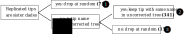
\includegraphics[scale=0.7]{figures/chart_phylorep}
\caption[Procedure followed to drop replicated tips from phylogenies]{\textbf{Procedure followed to drop replicated tips from phylogenies.} Most redundant tip labels were replicated twice. \textbf{(1)} When replicated tips were sister clades, the tips to drop were chosen randomly, as it did not affect the `true' phylogenetic position of the species; see case study 1 in Figure \ref{case1}. \textbf{(2)} When replicated were not sister clades, I kept the tip whose position was closest to the position of the same tip in the uncorrected tree (Figure \ref{case2}). \textbf{(3)} In a few cases, the corrected name did not appear in the original tree. Those were problematic cases, and the tips to drop were chosen randomly (Figure \ref{case3}). Nevertheless, occurences of that third case were rare.}
\label{chart_phylorep}
\end{figure}

% Replication in phylogenetic tips: case studies

\newpage
\paragraph{Case studies}

%%%% Case study 1
\subparagraph{Case study 1 (Figure \ref{case1}): replicated tips are sister clades.} In this example, Przewalski's toadhead agama (\textit{Phrynocephalus przewalskii}) figures in the original, uncorrected tree under two names identified as being synonyms (\textit{P. przewalskii} and \textit{P. frontalis}). As such, two replicated tips with the same name appear in the tree after the taxonomic correction. As they are sister clades, one tip is randomly dropped in the final corrected tree. In that case, the `true' phylogenetic position of the species is not affected.

\begin{figure}[h!]
\centering
\includegraphics[scale=0.7]{figures/Case_studies/Case1}
\caption[Phylogenetic trees before (A) and after (B) taxonomic correction, and after removing replicated tips (C) for species in the reptilian genus \textit{Phrynocephalus}]{\textbf{Phylogenetic trees before (A) and after (B) taxonomic correction, and after removing replicated tips (C) for species in the reptilian genus \textit{Phrynocephalus}.} The identified accepted name \textit{P. przewalskii}, in blue (A), is identified as being a synonym for \textit{P. frontalis,} which also figures in the uncorrected tree. As these clades are sister in the tree, one tip is dropped at random, and the final phylogenetic position of the species is not affected.}
\label{case1}
\end{figure}


%%%% Case study 2
\subparagraph{Case study 2 (Figure \ref{case2}): replicated tips are not sister clades, but the accepted name (tip label) figures in the original, uncorrected tree.} In that example, the amphibian species \textit{Ambystoma californiense} (California tiger salamander) was also found under its identified synonym \textit{A. tigrinum} in the original tree. In the final tree, the tip closest to the position of the same tip in the uncorrected tree was kept.

\begin{figure}[h!]
\centering
\includegraphics[scale=0.7]{figures/Case_studies/Case2}
\caption[Phylogenetic trees before (A) and after (B) taxonomic correction, and after removing replicated tips (C) for species in the amphibian genus \textit{Ambystoma}]{\textbf{Phylogenetic trees before (A) and after (B) taxonomic correction, and after removing replicated tips (C) for species in the amphibian genus \textit{Ambystoma}.} The identified accepted name \textit{A. californiense}, in blue (A), is identified as being a synonym for \textit{A. tigrinum,} which also figures in the uncorrected tree. There are not sister clades; in the final tree, the tip closest to the position of the same tip in the uncorrected tree was kept.}
\label{case2}
\end{figure}

%%%% Case study 3
\subparagraph{Case study 3 (Figure \ref{case3}): replicated tips are not sister clades, and the accepted name (tip label) does not figure in the original, uncorrected tree.} These were the problematic species listed in Table \ref{Phyrep}. In this example, the mammalian species \textit{Petinomys sagitta} (arrow flying squirrel) and  \textit{Hylopetes lepidus} (gray-cheeked flying squirrel)  have been identified to be synonymic, but the accepted name does not figure in the original tree. They are not sister clades; hence, one tip is randomly chosen to be dropped.

\begin{figure}[h!]
\centering
\includegraphics[scale=0.7]{figures/Case_studies/Case3}
\caption[Phylogenetic trees before (A) and after (B) taxonomic correction, and after removing replicated tips (C) for species in the mammalian genera \textit{Hylopetes} and \textit{Petinomys}]{\textbf{Phylogenetic trees before (A) and after (B) taxonomic correction, and after removing replicated tips (C) for species in the mammalian genera \textit{Hylopetes} and \textit{Petinomys}.} The identified accepted name \textit{H. sagitta}, in blue (B), does not figure in the uncorrected tree. It was identified to be the corresponding accepted name for \textit{P. sagitta} and \textit{H. lepidus}, which are not sister clades. One tip is randomly chosen to be dropped. Such cases were problematic but occurences were rare (Table \ref{Phyrep}).}
\label{case3}
\end{figure}

\pagebreak
\section{Trait coverage and completeness for PREDICTS species}
\begin{figure}[h!]
\centering
\includegraphics[scale=0.7]{figures/Predicts}
\caption[Trait coverage for species figuring in the PREDICTS database only]{\textbf{Trait coverage for species figuring in the PREDICTS database only.}}
\label{covPREDICTS}
\end{figure}

\begin{figure}[h!]
\centering
\includegraphics[scale=0.7]{figures/Traitcompleteness_PREDICTS}
\caption[Distribution of completeness values across species figuring in the PREDICTS database only]{\textbf{Distribution of completeness values across species figuring in the PREDICTS database only.} Completeness for reptilian and amphibian species figuring in the trait dataset particularly improved compared to the completeness for the whole dataset.}
\label{compPREDICTS}
\end{figure}

\section{Patterns in missing values with regards to phylogenetic trees}

\subsection{Within-family median completeness: plots with tip labels}

\subsubsection{Mammals}
\begin{figure}[h!]
\centering
\includegraphics[scale=0.55]{figures/NA_phylo_patterns/Mammals_completeness}
\caption[Within-family median completeness for mammals]{\textbf{Within-family median completeness for mammals.}}
\label{compPREDICTS}
\end{figure}

\subsubsection{Birds}
\begin{figure}[h!]
\centering
\includegraphics[scale=0.45]{figures/NA_phylo_patterns/Birds_completeness}
\caption[Within-family median completeness for birds]{\textbf{Within-family median completeness for birds.}}
\label{compPREDICTS}
\end{figure}

\subsubsection{Reptiles}
\begin{figure}[h!]
\centering
\includegraphics[scale=1.2]{figures/NA_phylo_patterns/Reptiles_completeness}
\caption[Within-family median completeness for reptiles]{\textbf{Within-family median completeness for reptiles.}}
\label{compPREDICTS}
\end{figure}

\subsubsection{Amphibians}
\begin{figure}[h!]
\centering
\includegraphics[scale=1.2]{figures/NA_phylo_patterns/Amphibians_completeness}
\caption[Within-family median completeness for amphibians]{\textbf{Within-family median completeness for amphibians.}}
\label{compPREDICTS}
\end{figure}

\pagebreak
\section{Missing values imputation}

\subsection{Phylogenetic signal}

\subsubsection{Significance}
\begin{figure}[h!]
\centering
\includegraphics[scale=0.75]{figures/Physignal/Allclasses}
\caption[Observed and simulated phylogenetic signals in categorical traits]{\textbf{Observed and simulated phylogenetic signals in categorical traits.} \textbf{(A)} Mammals; \textbf{(B)} birds; \textbf{(C)} reptiles; \textbf{(D)} amphibians. Black dots represent the observed phylogenetic signal in each categorical trait measured with $\delta$, a metric developed by Borges et al (2018). The observed measured is compared to the null distribution of $\delta$ (phylogenetic signal calculated when trait values are randomised). Blue points represent the median value of null $\delta$ expectations, and the blue error bars are 95\% confidence intervals. The null distribution of $\delta$ for each trait was generated by simulating 100 randomised trait vectors and calculating $\delta$ for each. As such, the median of null values represent the expected signal under a Brownian motion of trait evolution. Across all classes, all categorical traits presented significant phylogenetic signal. DA: diel activity; Sp: specialisation; TL: trophic level; PD: primary diet. Note that the phylogenetic signal of primary diet in mammals could not be calculated due to an implementation error.}
\label{Catphysig}
\end{figure}

\subsubsection{Phylogenetic signal computed with the original phylogenies}
\begin{table}[h!]
\renewcommand{\baselinestretch}{1}
\renewcommand{\arraystretch}{1.5}
\begin{center}\fontsize{9}{11}\selectfont
\caption[Phylogenetic signal in continuous and categorical traits and in range size, calculated with original phylogenies]{\textbf{Phylogenetic signal in continuous and categorical traits and in range size, calculated with original phylogenies.} \textbf{BM}: body mass; \textbf{L}: longevity; \textbf{LCS}: litter/clutch size; \textbf{HB}: habitat breadth; \textbf{DB}: diet breadth; \textbf{GL}: generation length; \textbf{BL}: body length; \textbf{SM}: sexual maturity; \textbf{RS}: range size; \textbf{TL}: trophic level; \textbf{PD}: primary diet; \textbf{DA}: diel activity; \textbf{Sp}: specialisation. The phylogenetic signal in continuous traits was calculated with Pagel's $\lambda$. For categorical traits, the $\delta$ metric developed by Borges et al (2018) was used. A star indicates a significant signal (significant p-values scores for the log-likelihood ratio test in the case of $\lambda$; and significant difference from the simulated null distribution of $\delta$ for categorical traits, see SI for test results). `na' are introduced for traits that were not considered in a class but may have been used in another as a predictor in missing values imputations. All traits showed significant phylogenetic signal, with signals for BM, L, LCS, and GL being particularly strong in mammals and birds (above 0.9). Here all calculations were conducted with the original phylogenies.} 
\label{physignal}
\begin{tabular}{|l|c|c|c|c|c|c|c|c|c|c|c|c|c|}
\hline
\multicolumn{1}{|c|}{\multirow{2}{*}{\textbf{Class}}} & \multicolumn{9}{c|}{\textbf{\begin{tabular}[c]{@{}c@{}}Continuous target traits,\\ additional predictors and range size: $\lambda$\end{tabular}}} & \multicolumn{4}{c|}{\textbf{\begin{tabular}[c]{@{}c@{}}Categorical traits:\\ $\delta$\end{tabular}}} \\ \cline{2-14} 
\multicolumn{1}{|c|}{}                                & \textbf{BM}    & \textbf{L}   & \textbf{LCS}   & \textbf{HB}   & \textbf{DB}   & \textbf{GL}   & \textbf{BL}   & \textbf{SM}   & \textbf{RS}   & \textbf{TL}           & \textbf{PD}           & \textbf{DA}                & \textbf{Sp}          \\ \hline
\textbf{Mammals}                                      & 1.0*           & 0.97*        & 0.96*          & 0.71*         & 0.99*         & 0.99*         & 1.0*          & na            & 0.98*         & 16*                   & 46*                   & 17*                        & 1.4*                 \\ \hline
\textbf{Birds}                                        & 1.0*           & 0.89*        & 0.92*          & 0.48*         & 0.49*         & 0.99*         & na            & na            & 0.66*         & 10*                   & 18*                   & 33$\cdot$10$^3$*           & 1.3*                 \\ \hline
\textbf{Reptiles}                                     & 0.69*          & 0.79*        & 0.76*          & 0.40*         & na            & na            & 1.0*          & 0.86*         & 0.56*         & 4.4*                  & na                    & 6.3*                       & 1.8*                 \\ \hline
\textbf{Amphibians}                                   & 0.72*          & 0.49*        & 0.58*          & 0.80*         & 0.52*         & na            & 0.96*         & na            & 0.62*         & 2.6*                  & 3.1*                  & 1.7*                       & 2.3*                 \\ \hline
\end{tabular}
\end{center}
\end{table}

%% table with p-values for log-likelihood ratio tests and wilcoxon signed rank tests


\pagebreak
\subsection{Imputation robustness}


\end{document}